\documentclass{llncs}
\usepackage[T1]{fontenc}
\usepackage{lmodern}
\usepackage{hyperref}
\usepackage{cite} % Multiple citations in one \cite command
\usepackage{pgfplotstable}
\usepackage{array} % Required for pgfplotstable dec sep align
\pgfplotsset{compat=1.12}
\usepackage{booktabs}

\usepackage{enumitem}
\setlist{parsep=0pt, listparindent=0.5cm}

\begin{document}
\title{A Comparison of Parallel Graph Processing Benchmarks}
\author{Samuel D. Pollard \and Boyana Norris}
\institute{University of Oregon \\
	Eugene OR 97403, USA \\
	\email{spollard@cs.uoregon.edu} \\
	\email{norris@cs.uoregon.edu}
}
\maketitle
\begin{abstract}
The increasing popularity of large network analysis problems has led to the emergence of many parallel and distributed graph processing systems---one survey in 2014 identified over 80. Since then, the landscape has evolved; some packages have become inactive while more are being developed. Determining the best approach for a given problem is infeasible for most developers. To enable easy, rigorous, and repeatable comparison of the capabilities of such systems, we present an approach and associated software for analyzing the performance and scalability of parallel, open-source graph libraries. We demonstrate our approach on five graph frameworks: GraphMat, the Graph500, the Graph Algorithm Platform, GraphBIG, and PowerGraph using synthetic and real-world datasets. We examine previously overlooked aspects of parallel graph processing performance such as phases of execution and energy usage for three algorithms: breadth first search, single source shortest paths, and PageRank and compare our results to Graphalytics.
\end{abstract}

\section{Introduction}

%% What's the problem (motivation)
Our research is motivated by the current state of parallel graph processing. The most comprehensive survey, released in 2014, identified and taxonomized over 80 different parallel graph processing systems without even including domain specific languages \cite{Doekemeijer:2015:GPFSurvey}.

An overarching issue among these systems is the lack of comprehensive comparisons. One possible reason is the considerable effort involved in getting each system to run: satisfying dependencies and ensuring data are correctly formatted are generally nontrivial tasks. Additionally, some systems are developed with large, multi-node clusters in mind while others only work with shared memory, single node computers. An example of the former is GraphX \cite{Xin:2013:GraphX}, which incurs some overhead while gaining fault tolerance and an example of the latter is Ligra \cite{Shun:2013:Ligra}, a framework requiring a shared-memory architecture.
% ``The project was motivated by the fact that the largest publicly available real-world graphs all fit in shared memory''

At the human level, there are optimizations for each system which may not be apparent. For example, the Parallel Boost Graph Library (PBGL) \cite{Gregor:2005:PBGL} provides generic implementations of their algorithms and the programmer must provide the template specializations. The optimal data structures may differ across algorithms and graphs and must be determined by the programmer.

%% How do we address it?
To mitigate the inherent bias in hand-generated implementations, all the experiments performed use the author-provided implementations; we assume the developers of each system will provide the most performant implementation. While this limits the scope of the experiments it mitigates the bias inherent in our programming skills.

%To address the challenges of getting various systems installed, we automate the process as much as possible n
%To showcase our methods we analyze the performance of several graph processing benchmarks to facilitate the selection among such systems. Our analysis is done with minimal source code modification.

Our contributions can be summarized as follows.
\begin{itemize}
	\item Automation of the installation, configuration, and dataset conversion to ensure the experiments execute in the same manner. Essentially, we provide a ``level playing field'' for graph algorithms.
	\item Comparison of algorithm runtime and scalability using a variety of data sets
	\item Comparison of our framework with the Graphalytics \cite{Capota:2015:Graphalytics} project
	\item Inspection of the source code of the surveyed parallel graph processing systems to ensure the same phases of execution are measured across differing execution and programming paradigms
	\item Provision of a experimental framework distinguishing between the data structure generation and algorithm execution phases of each system
	\item Analysis of energy consumption during the algorithm execution phase
\end{itemize}

\section{Related Work}
A related performance analysis project is Graphalytics \cite{Capota:2015:Graphalytics} which also attempts to automate the setup and execution of packages for performance analysis. However, in order for Graphalytics to analyze a graph processing system---Graphalytics calls these platforms---a programmer must implement Java classes as wrappers to call the particular implementations, satisfy dependencies, and set the correct shell commands to execute. These all require some knowledge of the inner workings of each system in addition to familiarity with the Graphalytics API.

The complexity of Graphalytics obfuscates the true behavior of the program. By default, Graphalytics generates an HTML report listing the runtimes for each dataset and each algorithm in seconds. For example, one run of a single source shortest paths algorithm took 5.6 seconds. However, perusing the log files reveals a more complete picture: of these 5.96 seconds, 0.21 was spent computing the shortest paths while the remaining time consisted of building the necessary data structures. Furthermore, data such as the number of iterations run for PageRank are not easily available using Graphalytics.
%We use GraphMat, the single source shortest paths algorithm, the dota-league dataset from the Game Trace Archive\cite{Guo:2012:GTA}, and the default settings as an example here.
% The full logs:
%Finished setting ids, time: 0.157009
%Starting sort
%Finished sort, time: 1.39571
%Finished setting edge pointers, time: 0.000133
%Starting build_dcsc
%Finished build_dcsc, time: 0.235948
%Finished setting ids, time: 0.154693
%Starting sort
%Finished sort, time: 1.75676
%Finished setting edge pointers, time: 0.000142
%Starting build_dcsc
%Finished build_dcsc, time: 0.238386
%Completed reading A from memory in 4.089144 seconds.
%Completed reading A from file in 5.114708 seconds
%Completed 19 iterations
%Timing results:
%- load graph: 5.11472 sec
%- initialize engine: 2.88486e-05 sec
%- run algorithm: 0.212451 sec
%- print output: 0.0799532 sec
%- deinitialize engine: 2.88486e-05 sec
%17:29:05.575 [INFO ] Benchmarking algorithm "Single source shortest paths" on graph "dota-league" took 5955 ms.

With a plugin to Graphalytics called Granula \cite{Ngai:2015:Granula} one can explicitly specify a performance model to analyze specific execution behavior such as the amount of communication or runtime of particular kernels of execution. This requires in-depth knowledge of the source code and execution model. Furthermore, creating such a model requires a high level of expertise with the given system and with Granula\footnote{An example of Granula can be seen at \url{https://github.com/tudelft-atlarge/graphalytics-platforms-graphx/tree/master/granula-model-graphx}}.

As with Graphalytics, the initial development effort is high but Granula paired with graphalytics allows automatic execution and compilation of performance results. Likewise, our approach provides automatic execution and performance analysis without requiring a performance and execution model for each system.

Other related work includes that of \cite{Satish:2014:NavigatingGraph}, which analyzes performance of several systems on datasets on the order of $30$ billion edges and \cite{Lu:2014:ExperimentalEval} which uses six real-world datasets and focuses on the vertex-centric programming model.

% The systems described in \cite{Doekemeijer:2015:GPFSurvey} operate with a wide range of parallelism paradigms and target architectures such as GPU \cite{Zhong:2014:Medusa, Kang:2009:Pegasus}, shared memory CPU \cite{Shun:2013:Ligra, kyrola:2012:Graphchi, Nguyen:2013:Galois}, a combination of CPU and GPU \cite{Gharaibeh:2012:Totem}, distributed filesystem based approaches \cite{Xin:2013:GraphX}, and distributed memory with MPI \cite{Gregor:2005:PBGL}.

% Beyond the systems described by Doekemeijer and Varbanescu, the problem has compounded with the addition of even more proprietary and open source projects such as \cite{Cheramangalath:2015:Falcon, Perez:2015:Ringo}, distributed memory approaches such as \cite{Hong:2015:PGX}. domain-specific languages \cite{Hong:2012:GreenMarl}, distributed database querying, \cite{Rodriguez:2015:Gremlin}, as well as novel communication schemes \cite{Edmonds:2013:ActiveMessages}. At the outset, this plethora of choices makes the question, ``which system is the best for my problem?'' daunting.

% In addition to libraries with associated APIs there has also been a propagation of ``reference implementations'' which implement the most common graph algorithms such as \cite{Beamer:2015:GAPBench, Nai:2015:Graphbig}. Thus, even selecting a standard and a benchmark over which to compare various implementations is nontrivial. To quote Andrew Tanenbaum, ``The nice thing about standards is that you have so many to choose from.''

\section{Experimental Setup}

\subsection{Graph Processing Systems}

This report explores four shared memory parallel graph processing platforms. The first three are so-called ``reference implementations'' while the remaining two are included because of their performance and popularity. Our target is shared memory CPU processing. Other popular libraries such as the Parallel Boost Graph Library \cite{Gregor:2005:PBGL} are not considered here because the authors do not provide reference implementations. The systems are:

\begin{enumerate}
	\item The Graph500\footnote{We used the most recent version from \url{https://github.com/graph500/graph500}, most similar to release 2.1.4.} \cite{Murphy:2010:Graph500}
	\item The Graph Algorithm Platform (GAP) Benchmark Suite \cite{Beamer:2015:GAPBench}
	\item GraphBIG \cite{Nai:2015:Graphbig}
	\item GraphMat \cite{Sundaram:2015:GraphMat}
	\item PowerGraph \cite{Gonzalez:2012:Powergraph}
\end{enumerate}

\subsection{Algorithms}

We consider three algorithms though not all algorithms are available on all systems.

\begin{enumerate}
	\item Breadth First Search (BFS)
	\item Single Source Shortest Paths (SSSP)
	\item PageRank
\end{enumerate}

The canonical performance leaderboard for parallel graph processing is the Graph500 \cite{Murphy:2010:Graph500}. The advantage of the Graph500 is it provides standardized measurement specifications and dataset generation. The primary drawback with the Graph500 is it measures a single algorithm: BFS.

Our work aims to add similar rigor to other graph algorithms by borrowing heavily from the Graph500 specification. The Graph500 Benchmark 1 (``Search'') is concerned with two kernels: the creation of a graph data structure from an edge list stored in RAM and the actual BFS\footnote{For a complete specification, see \url{http://graph500.org/specifications}}. We run the BFS using 32 random roots.

One straightforward extension to BFS and our second algorithm is the Single-Source Shortest Paths algorithm (SSSP). We use the same graph and the same source vertices as in BFS.

The third algorithm is PageRank. These three algorithms are used because of their popularity; most libraries provide reference implementations.

\subsection{Machine Specifications}
Table~\ref{tab:specs} shows the specifications of the research computer.

\begin{table}
	\centering
	\caption{The operating system is GNU/Linux version 4.4.0-22. The disparity between the CPU's advertised clock speed and the ``CPU Clock'' row is a result of the Turbo Boost technology which can increase the clock speed to a limit. We use the manufacturer's published maximum clock speeds which can be found at \url{http://ark.intel.com}.}
	% For arya I deleted Max RAM Freq	2133MHz
	\pgfplotstabletypeset[
	header=false,
	col sep=tab,
	string type,
	every head row/.style={output empty row, before row=\bottomrule},
	columns/0/.style={column type={|r|}},
	columns/1/.style={column type={l|}},
	every last row/.style={after row=\toprule},
	]{../report/specs.csv}
	\label{tab:specs}
\end{table}

\subsection{Datasets}
We use the Graph500 synthetic graph generator which creates a Kronecker graph \cite{Leskovec:2010:Kronecker} with initial parameters of $A = 0.57, B = 0.19, C = 0.19,$ and $D = 1-(A+B+C) = 0.05$.

The Graphalytics results in Table~\ref{tab:graphalytics} were performed on the Dota-League dataset. This dataset contains 61,670 vertices and 50,870,313 edges. This dataset is sourced from the Game Trace Archive\cite{Guo:2012:GTA} and modified for Graphalytics\footnote{This dataset is available at \url{https://atlarge.ewi.tudelft.nl/graphalytics/}.}.

\section{Performance Analysis}

\subsection{Runtime}

In Table~\ref{tab:graphalytics} we show the results from running Graphalytics on a single dataset. For an explanation of each algorithm used, see \cite{Iosup:2016:Graphalyticstech}. Table~\ref{tab:graphalytics} shows only a broad overview of the two systems: GraphBIG and PowerGraph. In general, we see GraphBIG is more performant. However, results such as these are preliminary and do not show the complete picture.

%Table~\ref{tab:perf} lists performance in milliseconds of runtime according to the graphalytics output. Graphalytics also outputs MTEPS or millions of traversed edges pers econd. However, the graphalytics version does not make sense in all cases: for example, computing the local clustering coefficient involves traversing each edge multiple times (proportional to the sparsity of the graph), while BFS traverses each edge exactly once, and the number of edges traversed with PageRank depends on the connectivity of the graph and the number of iterations.

\begin{table}
% ,graphmat,openg,powergraph
%	Community Detection,0,212.5,1167
%	PageRank,0,293.5,983
%	Local Clustering Coefficient,0,316.5,1011
%	Weakly Connected Components,0,89,767.5
%	Single-Source Shortest Paths,11298.5,6378.5,34654.5
	\caption{Performance results are in milliseconds. Community detection is performed using label propagation. At the time of this writing, Graphalytics only supports SSSP for GraphMat.}
	\centering
	\pgfplotstabletypeset[
		col sep=comma,
		columns={[index]0,graphmat,openg,powergraph},
		every head row/.style={after row=\midrule},
		columns/0/.style={string type, column type={l|}, column name={}},
		columns/graphmat/.style={
			column name={GraphMat},
			string replace={0}{},
			dec sep align,
			empty cells with={N/A}
		},
		columns/openg/.style={
			column name={GraphBIG},
			dec sep align},
		columns/powergraph/.style={
			column name={PowerGraph},
			dec sep align}
	]{../report/runtime.csv}
	\label{tab:graphalytics}
\end{table}

Table~\ref{tab:epg-perf}, in contrast, gives an overview of the performance results of running graphalytics and our approach using the same dataset [TODO: Get the Dota-League Dataset working with eas-parallel-graph and replace Table~\ref{epg-perf}]. Table~\ref{tab:epg-perf} shows the average time across 32 roots, whereas Graphalytics by default shows results for a single root.

Further detail is shown in Figs.~\ref{fig:bfs-time} and \ref{fig:sssp-time}, giving box plots for the runtime distributions. However, even these do not give a complete picture of performance. Both of these show GraphMat to not be highly performant. However, a likely explanation is that GraphMat's underlying computation model (sparse matrix operations) paired the increased overhead of GraphMat's doubly-compressed sparse row (DSCR) graph representation is more conducive to larger-scale graphs.

%\begin{table}
%	\centering
%	\begin{tabular}{l|c|c|c}
%		System & Load Graph & \begin{tabular}[x]{@{}c@{}}Construct Data \\ Structure\end{tabular} & Run BFS \\ \hline
%		Graph500 & 0.3474 & 0.3971 & 0.003380 \\
%		GAP      & 2.351  & 0.1935 & 0.001393 \\
%		GraphMat & 0.1511 & 1.101  & 0.1031 \\
%		GraphBIG & 37.22  & N/A    & 0.1528 \\
%	\end{tabular}
%	\caption{This table shows times for $2^{20}$ verties and the times are in seconds. The Graph500 generates the graph instead of loading it into a file. GraphBIG builds the graph and reads in the file simultaneously. These results were averaged across 32 roots.}
%	\label{tab:epg-perf}
%\end{table}

\begin{figure}
	\centering
	\caption{The $y$-axis is logarithmic. GraphBIG reads in the file and generates the data structure simultaneously so is omitted.}
	\begin{minipage}{0.48\linewidth}
		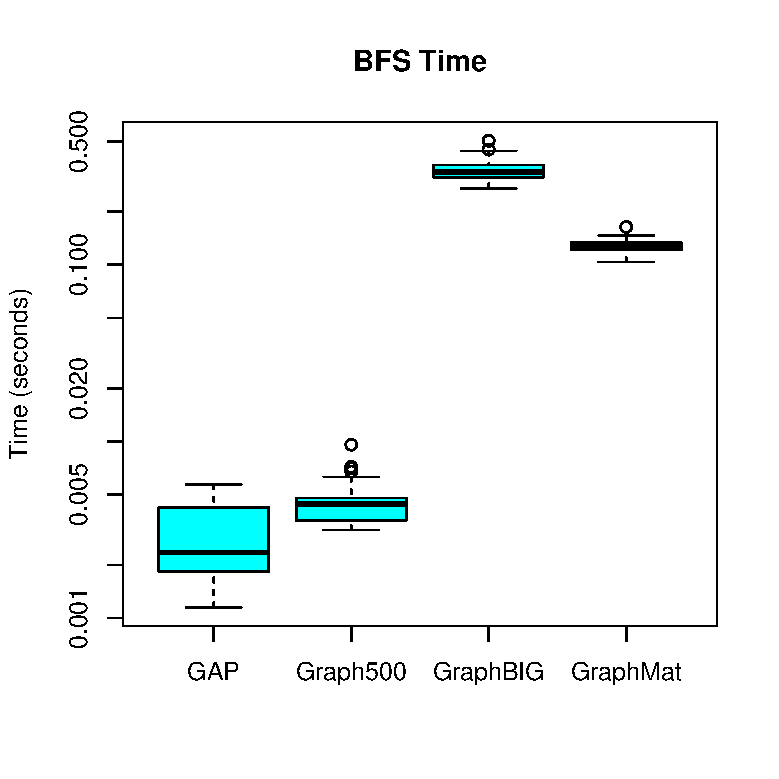
\includegraphics[width=\linewidth, trim=0 36pt 18pt 0, clip]{graphics/bfs_time.pdf}
	\end{minipage}
	\begin{minipage}{0.48\linewidth}
		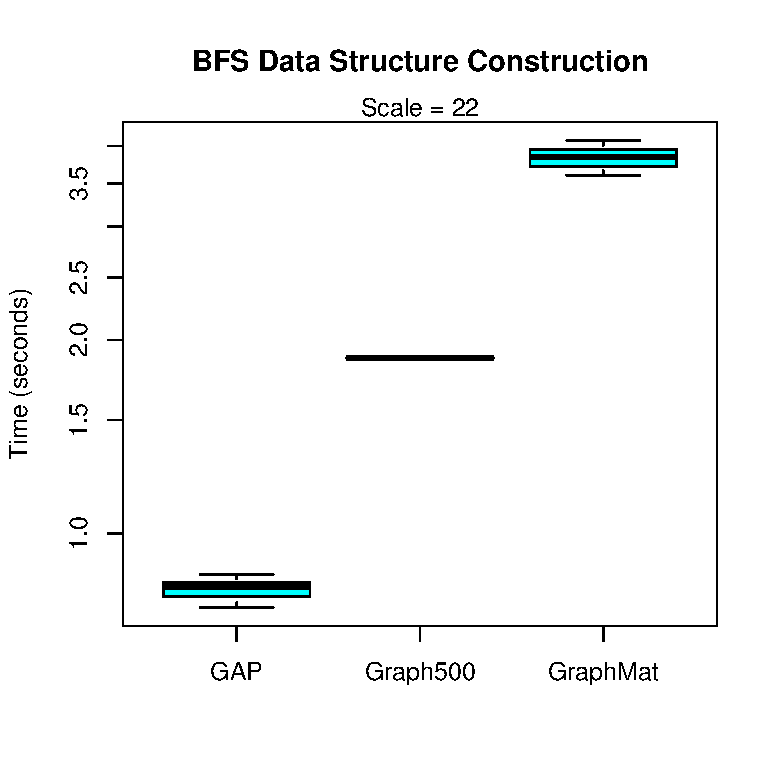
\includegraphics[width=\linewidth, trim=0 36pt 18pt 0, clip]{graphics/bfs_dsc.pdf}
	\end{minipage}
	\label{fig:bfs-time}
\end{figure}

\begin{figure}
	\centering
	\begin{minipage}{0.59\linewidth}
		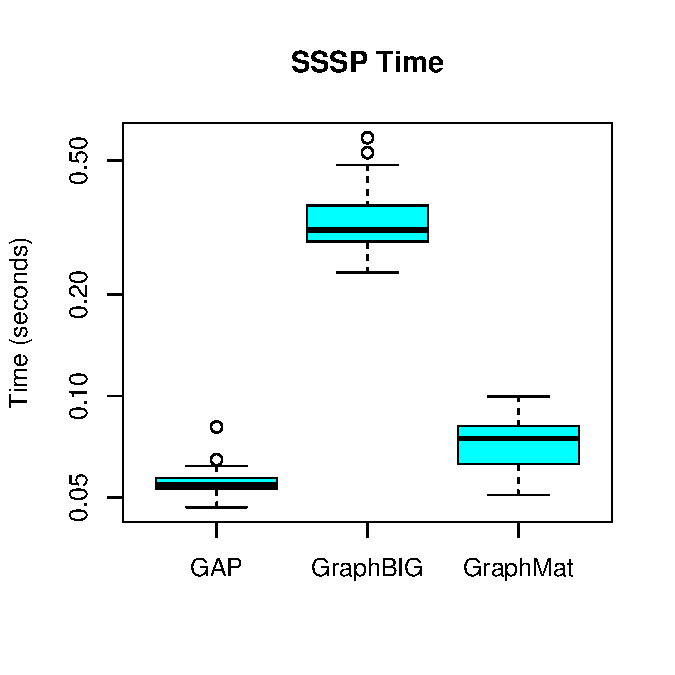
\includegraphics[width=\linewidth, trim=0 36pt 18pt 0, clip]{graphics/sssp_time.pdf}
	\end{minipage}
	\begin{minipage}{0.365\linewidth}
		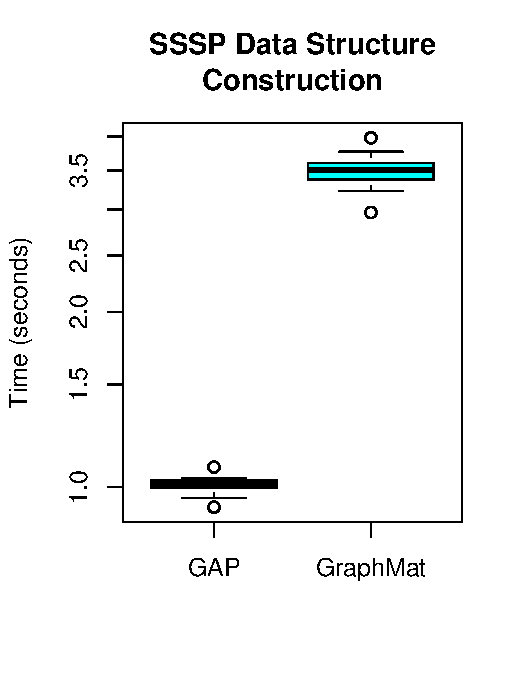
\includegraphics[width=\linewidth, trim=0 36pt 18pt 0, clip]{graphics/sssp_dsc.pdf}
	\end{minipage}
	\caption{The $y$-axis is logarithmic. Both PowerGraph and GraphBIG construct their data structures at the same time as they read in the file.}
	\label{fig:sssp-time}
\end{figure}

The behavior of PageRank is slightly different. As with SSSP and BFS, the GAP Benchmark Suite is the fastest, and it also requires the fewest iterations. While care was taken to ensure the same stopping criterion is met, the particular implementation methods make it impossible to ensure the same computations are taking place. In general, we measured $\sum_{k=1}^{n} |p_k^{(i)} - p_k^{(i-1)}|$ where $i$ is the iteration and $n$ is the number of vertices, both the vertex-centric approaches, PowerGraph and GraphMat, take more iterations.

\begin{figure}
	\centering
	\begin{minipage}{0.48\linewidth}
		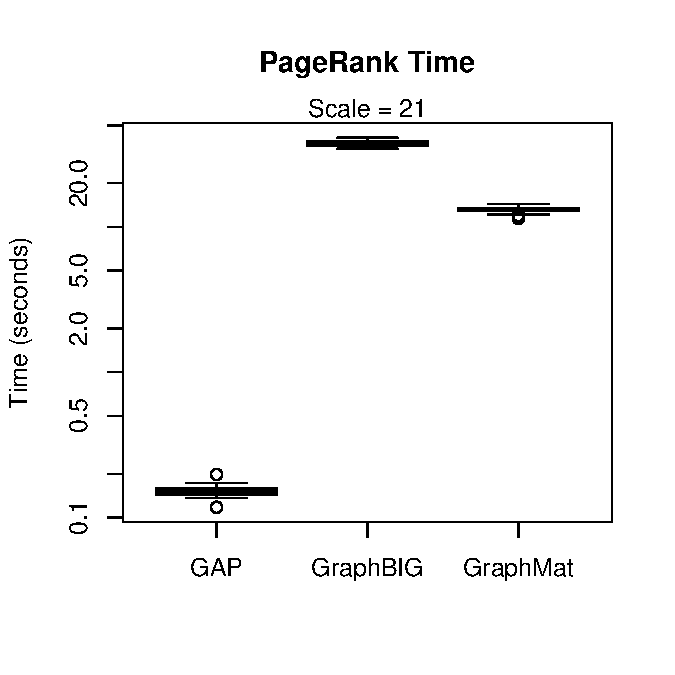
\includegraphics[width=\linewidth, trim=0 18pt 18pt 0, clip]{graphics/pr_time.pdf}
	\end{minipage}
	\begin{minipage}{0.48\linewidth}
		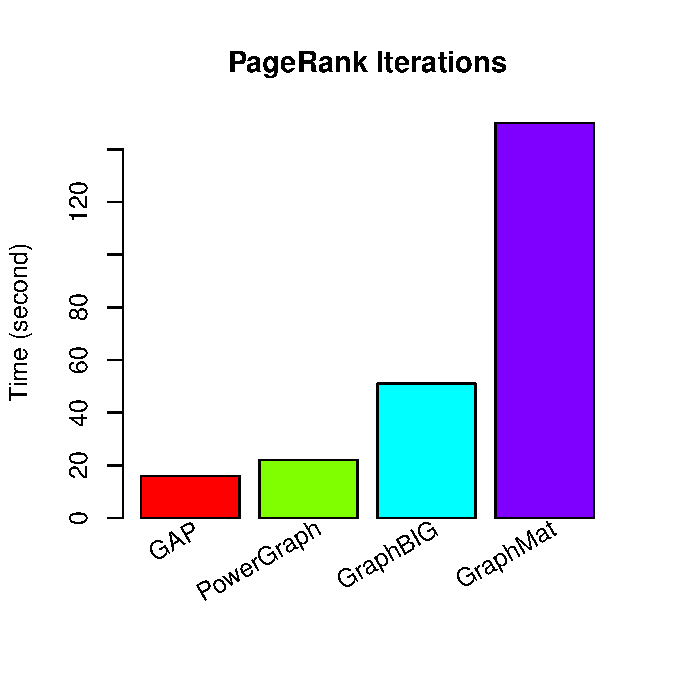
\includegraphics[width=\linewidth, trim=0 18pt 18pt 0, clip]{graphics/pr_iters.pdf}
	\end{minipage}
	\caption{The $y$-axis is logarithmic only for the left figure. GraphMat continues to run until none of the vertices' ranks change. GraphMat iterations are measured differently because of the ``think like a vertex'' paradigm and runs until none of the vertices' ranks change. For the others, we use the stopping condition that the sum of the changes in the weights is no more than $6 \times 10^{-8}$, or approximately machine epsilon for single precision floating point numbers.}
	\label{fig:pr}
\end{figure}

\begin{figure}
	\centering
	\begin{minipage}{0.48\linewidth}
		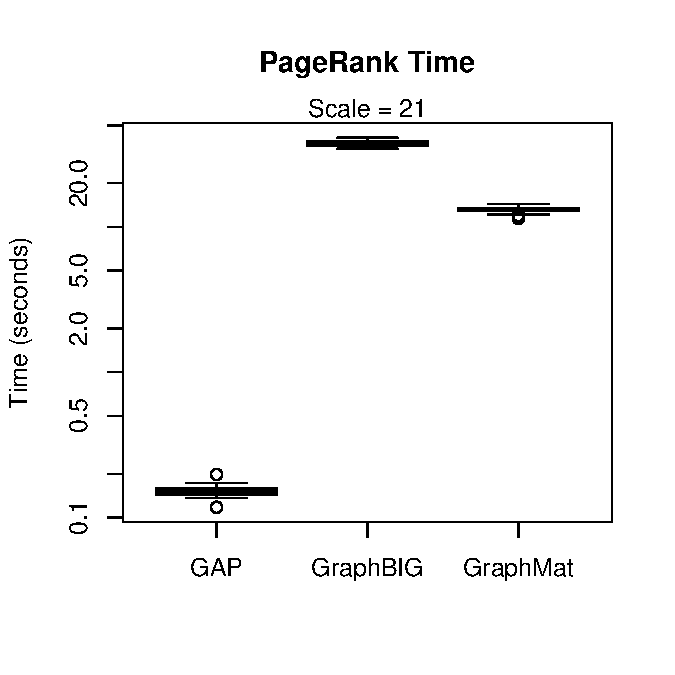
\includegraphics[width=\linewidth, trim=0 24pt 18pt 0, clip]{graphics/pr_time.pdf}
	\end{minipage}
	\begin{minipage}{0.48\linewidth}
		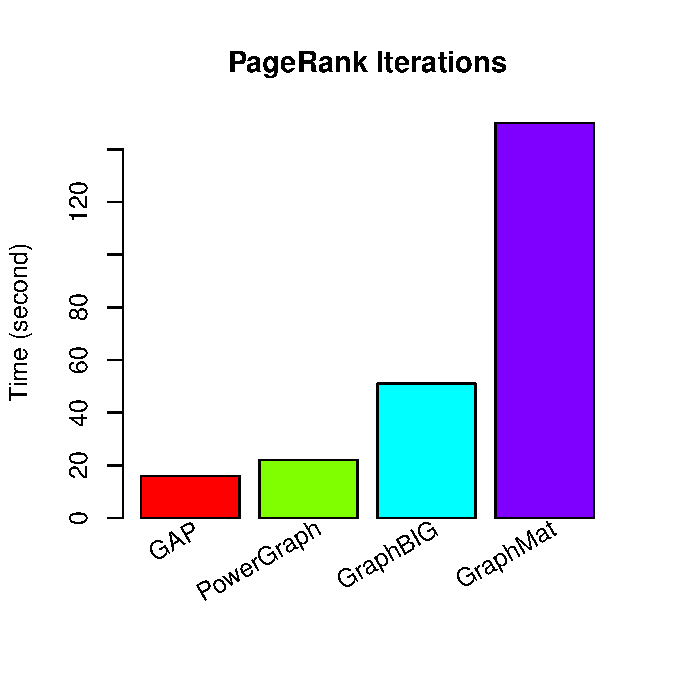
\includegraphics[width=\linewidth, trim=0 24pt 18pt 0, clip]{graphics/pr_iters.pdf}
	\end{minipage}
	\caption{The $y$-axis is logarithmic. GraphMat iterations are measured differently because of the ``think like a vertex'' paradigm and runs until none of the vertices' ranks change.}
	\label{fig:pr}
\end{figure}

The challenge in comparing iteration counts for PageRank underscores an important challenge for any comparison of graph processing systems. The assumptions under which the various platforms operate can have a dramatic effect on the program. For example, the GAP Benchmark Suite stores vertex weights as 32-bit integers. However, other systems store them as floating point numbers. This may affect performance in addition to runtime behavior in cases where weights like $0.2$ are cast to $0$. Similarly, how a grpah is represented in the system (e.g. weighed or directed) may have performance and algorithmic implications but is not always readily apparent.

In Fig.~\ref{fig:bfs-scaling}, we see BFS scalability\dots
\begin{figure}
	\centering
	\begin{minipage}{0.55\linewidth}
		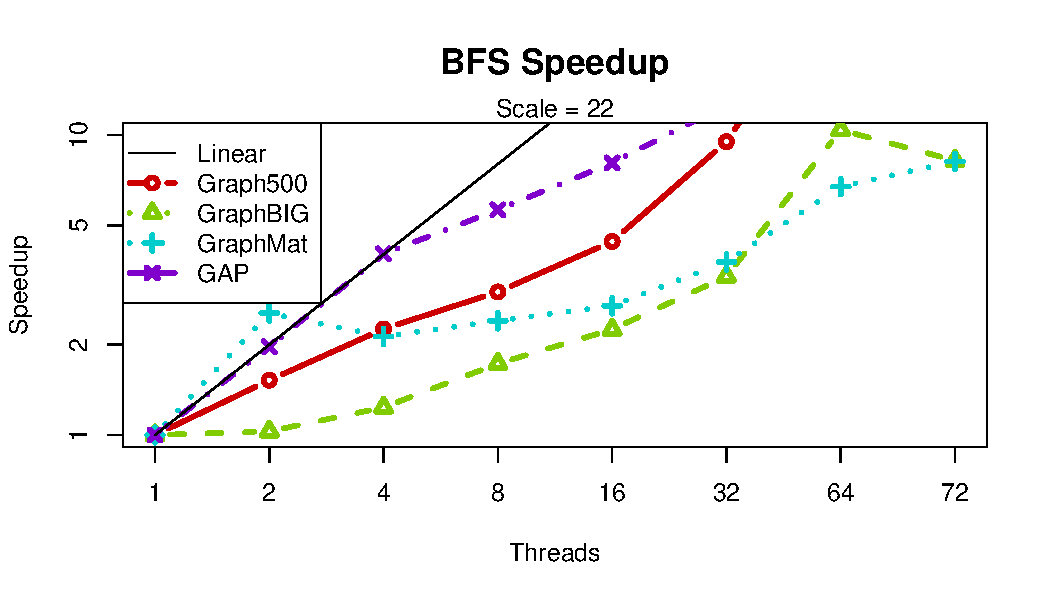
\includegraphics[width=\linewidth, trim=0 18pt 18pt 0, clip]{graphics/bfs_speedup.pdf}
	\end{minipage}
	\begin{minipage}{0.425\linewidth}
		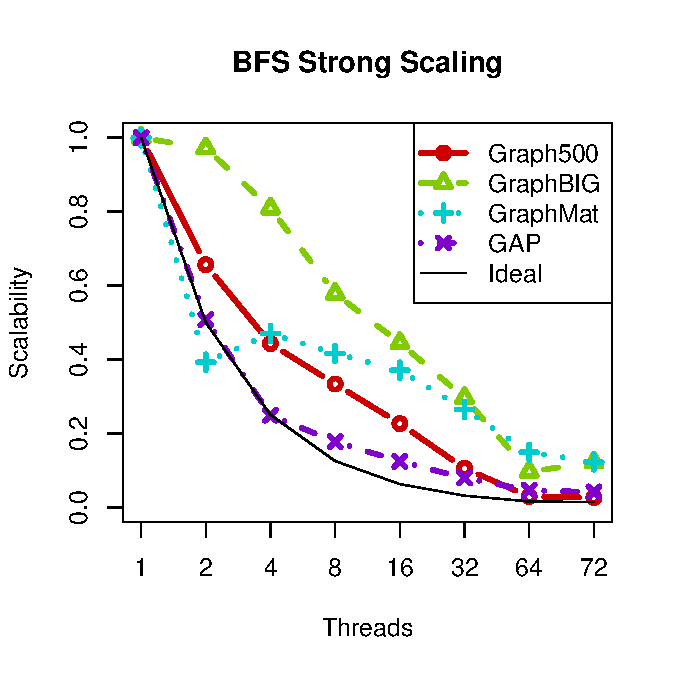
\includegraphics[width=\linewidth, trim=0 18pt 18pt 0, clip]{graphics/bfs_ss.pdf}
	\end{minipage}
	\caption{Both figures use the kronecker graph with $2^{20}$ vertices with an average of 16 edges per vertex.}
	\label{fig:bfs-scaling}
\end{figure}

\subsection{Power and Energy Consumption}
We use the Performance Application Programming Interface (PAPI) \cite{Browne:2000:PAPI} to gain access to Intel's Running Average Power Limit (RAPL), which provides access to a set of hardware counters measuring energy usage. PAPI provides convenient access to these values and average energy in nanojoules for a given time interval. We modify the source code for each project to time only the actual BFS computation. In our case, the fastest code is also the most energy efficient, though with this level of granularity we could detect circumstances where one could make a tradeoff between energy and runtime.

\begin{table}
	\caption{The data are generated from a Kronecker graph with $2^{22}$ vertices. Sleeping Energy refers to the power (in Watts) consumed during the Unix \texttt{sleep} function, multiplied by time. Effectively, this measures the amount of energy that would have been consumed even if nothing was running. The increase over sleep is the ratio of the first and third columns. These are all averaged over the 32 roots.}
	\centering
	\begin{tabular}{l|r|r|r|r}
			&	GAP  &    Graph500 & GraphBIG & GraphMat \\ \hline
		Time (s) &  0.01636 & 0.01884 & 1.600 & 1.424 \\
		Average Power per Root (W) & 72.38 & 97.17 & 78.01 & 70.12 \\
		Energy per Root (J) &	1.184 & 1.830 & 112.213 & 111.104 \\
		Sleeping Energy (J) & 0.4046  & 0.4660 & 39.591 &  35.234 \\
		Increase over Sleep & 2.926 & 3.928 & 2.834 & 3.153
	\end{tabular}
\end{table}

RAPL also allows the measurement of DRAM power and energy, whose results are shown in Fig.~\ref{fig:ram-power}.

\begin{figure}
	\centering
	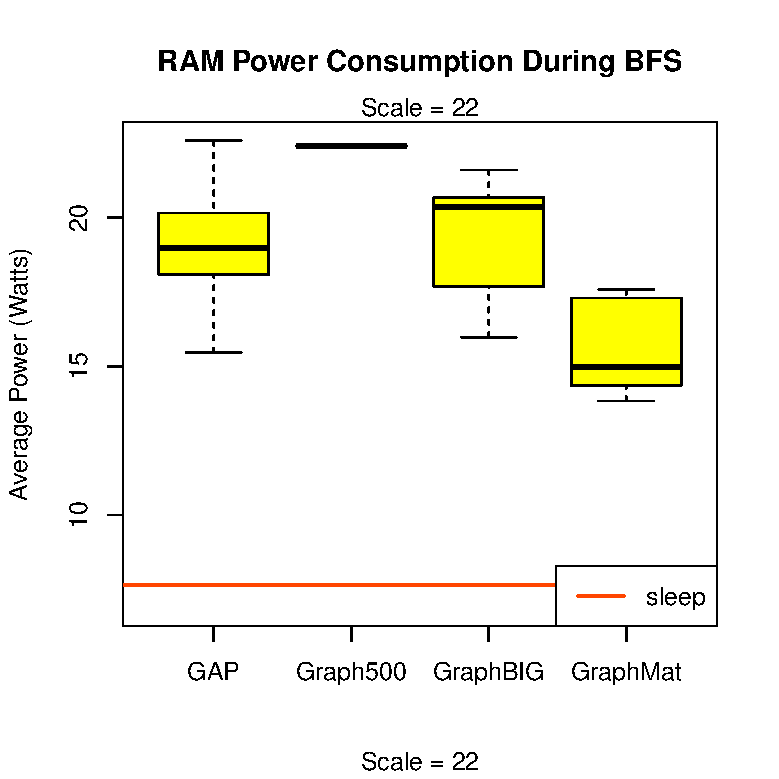
\includegraphics[width=0.6\linewidth, trim=0 36pt 18pt 0, clip]{graphics/bfs_ram_power.pdf}
	\caption{RAM Power Consumption, averaged across all roots. [TODO: Explain more]}
	\label{fig:ram-power}
\end{figure}

\section{Future Work and Conclusion}
The problem of choosing a system for graph processing at large scale is far from being simple. We make our code available at \url{https://github.com/HPCL/easy-parallel-graph} and encourage further experimentation. Our results required minor changes to the original projects to add calls to PAPI sampling and those changes are also available on forked versions of the repositories.

Overall, the GAP Benchmark Suite was the highest-performing system across the given datasets and the most scalable. However, this is only for relatively small graphs; all the graphs used here had at most $2^{22}$ vertices. It should be noted that GAP is also the most recent of projects. Thus, we recommend graph processing algorithm designers compare their implementations against the GAP Benchmark Suite to as a good test of performance.

There are a vast number of directions this work could go. To ensure fairness, each platform must be configured to use the same graphs and the same roots. In the case of GraphBIG this required the file to be loaded in for each experiment. This was by far the most time consuming of the experiments; the file reading for GraphBIG being done serially on an uncompressed ASCII text format for graphs. This limited the sizes of the experiments we could run. Graphalytics also had circumstances with the more computationally expensive algorithms  where certain experiments fail \cite{Iosup:2016:Graphalyticstech}, so determining whether an algorithm will finish given a particular machine, input size, runtime limit, and resources is an important unanswered question.

\bibliographystyle{splncs03}
\bibliography{../drp}
\end{document}
